\begin{figure*}[hbtp]
  \centering
  \subfigure[Initial graph]{
    \label{fig:about-frontier-df1}
    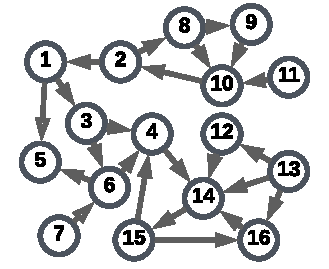
\includegraphics[width=0.23\linewidth]{out/about-frontier-11.pdf}
  }
  \subfigure[Marking initial affected vertices (DF)]{
    \label{fig:about-frontier-df2}
    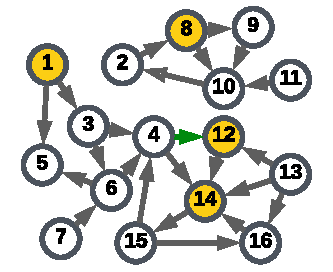
\includegraphics[width=0.23\linewidth]{out/about-frontier-32.pdf}
  }
  \subfigure[After first iteration (DF)]{
    \label{fig:about-frontier-df3}
    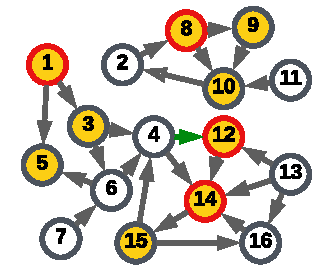
\includegraphics[width=0.23\linewidth]{out/about-frontier-33.pdf}
  }
  \subfigure[After second iteration (DF)]{
    \label{fig:about-frontier-df4}
    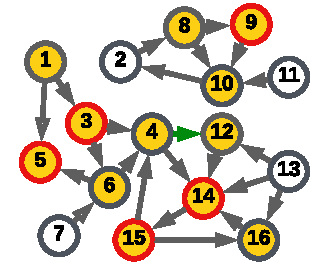
\includegraphics[width=0.23\linewidth]{out/about-frontier-34.pdf}
  } \\[2ex]
  \subfigure[Initial graph]{
    \label{fig:about-frontier-dfp1}
    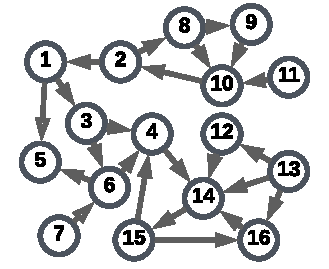
\includegraphics[width=0.23\linewidth]{out/about-frontier-11.pdf}
  }
  \subfigure[Marking initial affected vertices (DF-P)]{
    \label{fig:about-frontier-dfp2}
    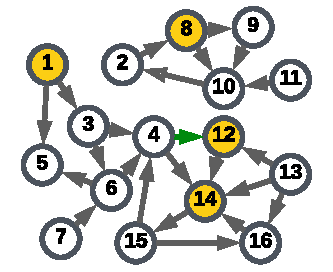
\includegraphics[width=0.23\linewidth]{out/about-frontier-32.pdf}
  }
  \subfigure[After first iteration (DF-P)]{
    \label{fig:about-frontier-dfp3}
    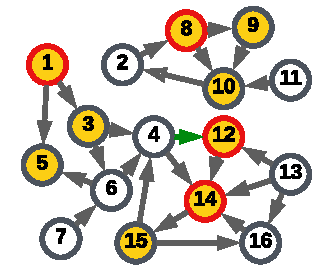
\includegraphics[width=0.23\linewidth]{out/about-frontier-33.pdf}
  }
  \subfigure[After second iteration (DF-P)]{
    \label{fig:about-frontier-dfp4}
    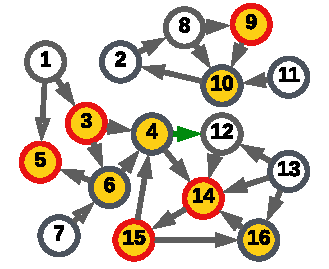
\includegraphics[width=0.23\linewidth]{out/about-frontier-44.pdf}
  } \\[2ex]
  \subfigure[Initial graph]{
    \label{fig:about-frontier-dt1}
    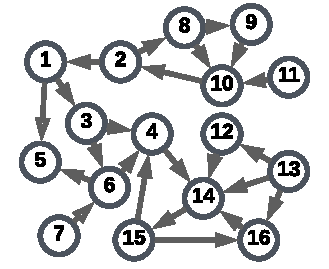
\includegraphics[width=0.23\linewidth]{out/about-frontier-11.pdf}
  }
  \subfigure[Marking affected vertices (DT)]{
    \label{fig:about-frontier-dt2}
    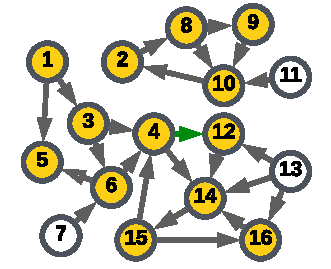
\includegraphics[width=0.23\linewidth]{out/about-frontier-22.pdf}
  }
  \subfigure[After first iteration (DT)]{
    \label{fig:about-frontier-dt3}
    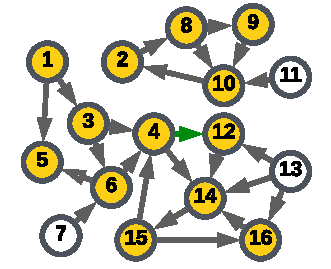
\includegraphics[width=0.23\linewidth]{out/about-frontier-22.pdf}
  }
  \subfigure[After second iteration (DT)]{
    \label{fig:about-frontier-dt4}
    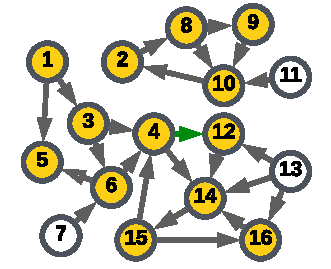
\includegraphics[width=0.23\linewidth]{out/about-frontier-22.pdf}
  } \\[-2ex]
  \caption{An illustration of our \textit{Dynamic Frontier (DF)} and \textit{Dynamic Frontier with Pruning (DF-P)} approaches, in subfigures (a)-(d) and (e)-(h) respectively, compared against the \textit{Dynamic Traversal (DT)} approach, shown in subfigures (i)-(l) \cite{sahu2024df}.}
  \label{fig:about-frontier}
\end{figure*}
